\documentclass[tikz,border=10pt]{standalone}
\usepackage{pgfplots}
\usepgfplotslibrary{fillbetween}
\usetikzlibrary{patterns}
\pgfplotsset{every axis plot post/.append style =
  {samples=80, smooth, thick, black, mark=none} }
\begin{document}
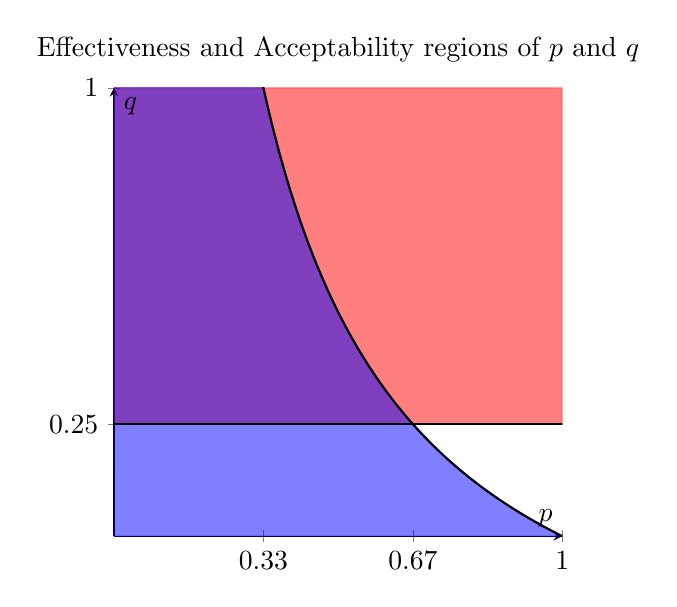
\begin{tikzpicture}
\begin{axis}[axis lines = center,
  title={Effectiveness and Acceptability regions of $p$ and $q$},
  xlabel=$p$, ylabel=$q$,
  ytick={0,0.25,1},
  xtick={0,1/3,2/3,1},
  axis equal image, domain = 0:1, ymax=1]
  \addplot[name path=acceptable] {(1-x)/(2*x)};
  \addplot[name path=effective] {1/4};
  \path[name path=xaxis] (axis cs:0,0) -- (axis cs:1,0);
  \path[name path=ylim] (axis cs:0,1) -- (axis cs:1,1);
  \addplot[color=red, draw=red,
           opacity=0.5]
    fill between[of=effective and ylim];
  \addplot[color=blue, draw=blue,
    opacity=0.5]
    fill between[of=acceptable and xaxis];
\end{axis}
\end{tikzpicture}
\end{document}